\documentclass{beamer}

\mode<presentation> {
  \usetheme{Luebeck}   % Luebeck, Malmoe, Dresden, Warsaw
  \setbeamercovered{transparent=35}
  %\usecolortheme{seagull}  % seagull, seahorse
}

\usepackage[utf8]{inputenc}
\usepackage[czech]{babel}
\usepackage{palatino}
\usepackage{graphicx}

\usepackage{listings}
\lstset{ %
  basicstyle=\small\ttfamily,        % the size of the fonts that are used for the code
  aboveskip={1pt plus 1pt minus 1pt},
  belowskip={1pt plus 1pt minus 1pt},
  breakatwhitespace=false,         % sets if automatic breaks should only happen at whitespace
  breaklines=true,                 % sets automatic line breaking
  captionpos=n,                    % sets the caption-position to bottom
  escapeinside={\%*}{*)},          % if you want to add LaTeX within your code
  extendedchars=true,              % lets you use non-ASCII characters; for 8-bits encodings only, does not work with UTF-8
  frame=none,	                   % adds a frame around the code
  keepspaces=true,                 % keeps spaces in text, useful for keeping indentation of code (possibly needs columns=flexible)
  numbers=none,                    % where to put the line-numbers; possible values are (none, left, right)
  numbersep=8pt,                   % how far the line-numbers are from the code
  numberstyle=\footnotesize\color{gray}, % the style that is used for the line-numbers
  rulecolor=\color{black},         % if not set, the frame-color may be changed on line-breaks within not-black text (e.g. comments (green here))
  showspaces=false,                % show spaces everywhere adding particular underscores; it overrides 'showstringspaces'
  showstringspaces=false,          % underline spaces within strings only
  showtabs=false,                  % show tabs within strings adding particular underscores
  stepnumber=1,                    % the step between two line-numbers. If it's 1, each line will be numbered
  tabsize=2,	                   % sets default tabsize to 2 spaces
  title=\lstname,                   % show the filename of files included with \lstinputlisting; also try caption instead of title
  xleftmargin=\parindent,
  numberbychapter=false
}

\usepackage[skip=0pt]{caption}

\usepackage{tikz}
\usepackage{transparent}

\begin{document}
%\setbeamertemplate{caption}{\insertcaption}

\title[\textbf{Editor konfiguračních souborů Flow123d}]{Editor konfiguračních souborů Flow123d}
\subtitle{Úvodní prezentace}
\author[\textbf{Bc. Tomáš Křížek}]{{\large Bc. Tomáš Křížek}\\{\scriptsize Vedoucí práce: doc. Jiřina Královcová}}
\institute[TUL]{Technická univerzita v Liberci}
\date{1.~března~2016}

\begin{frame}
	\titlepage
\end{frame}

\begin{frame}
	\frametitle{Osnova prezentace}
	\begin{itemize}
		\item Simulátor Flow123d
		\item Zadávání výpočetních úloh
		\item Problémy s konfiguračními soubory
		\item Editor konfiguračních souborů
	\end{itemize}
\end{frame}

\begin{frame}[t]
	\vspace{0.5cm}
	\frametitle{Simulátor Flow123d}
	\begin{itemize}[<+>]
		\item modelování procesů v horninovém prostředí
		\item výpočetně náročné
		\item pouze textové rozhraní
	\end{itemize}
	\vspace{0.4cm}
	\begin{figure}[h]
	\only<1-3>{\transparent{0.35}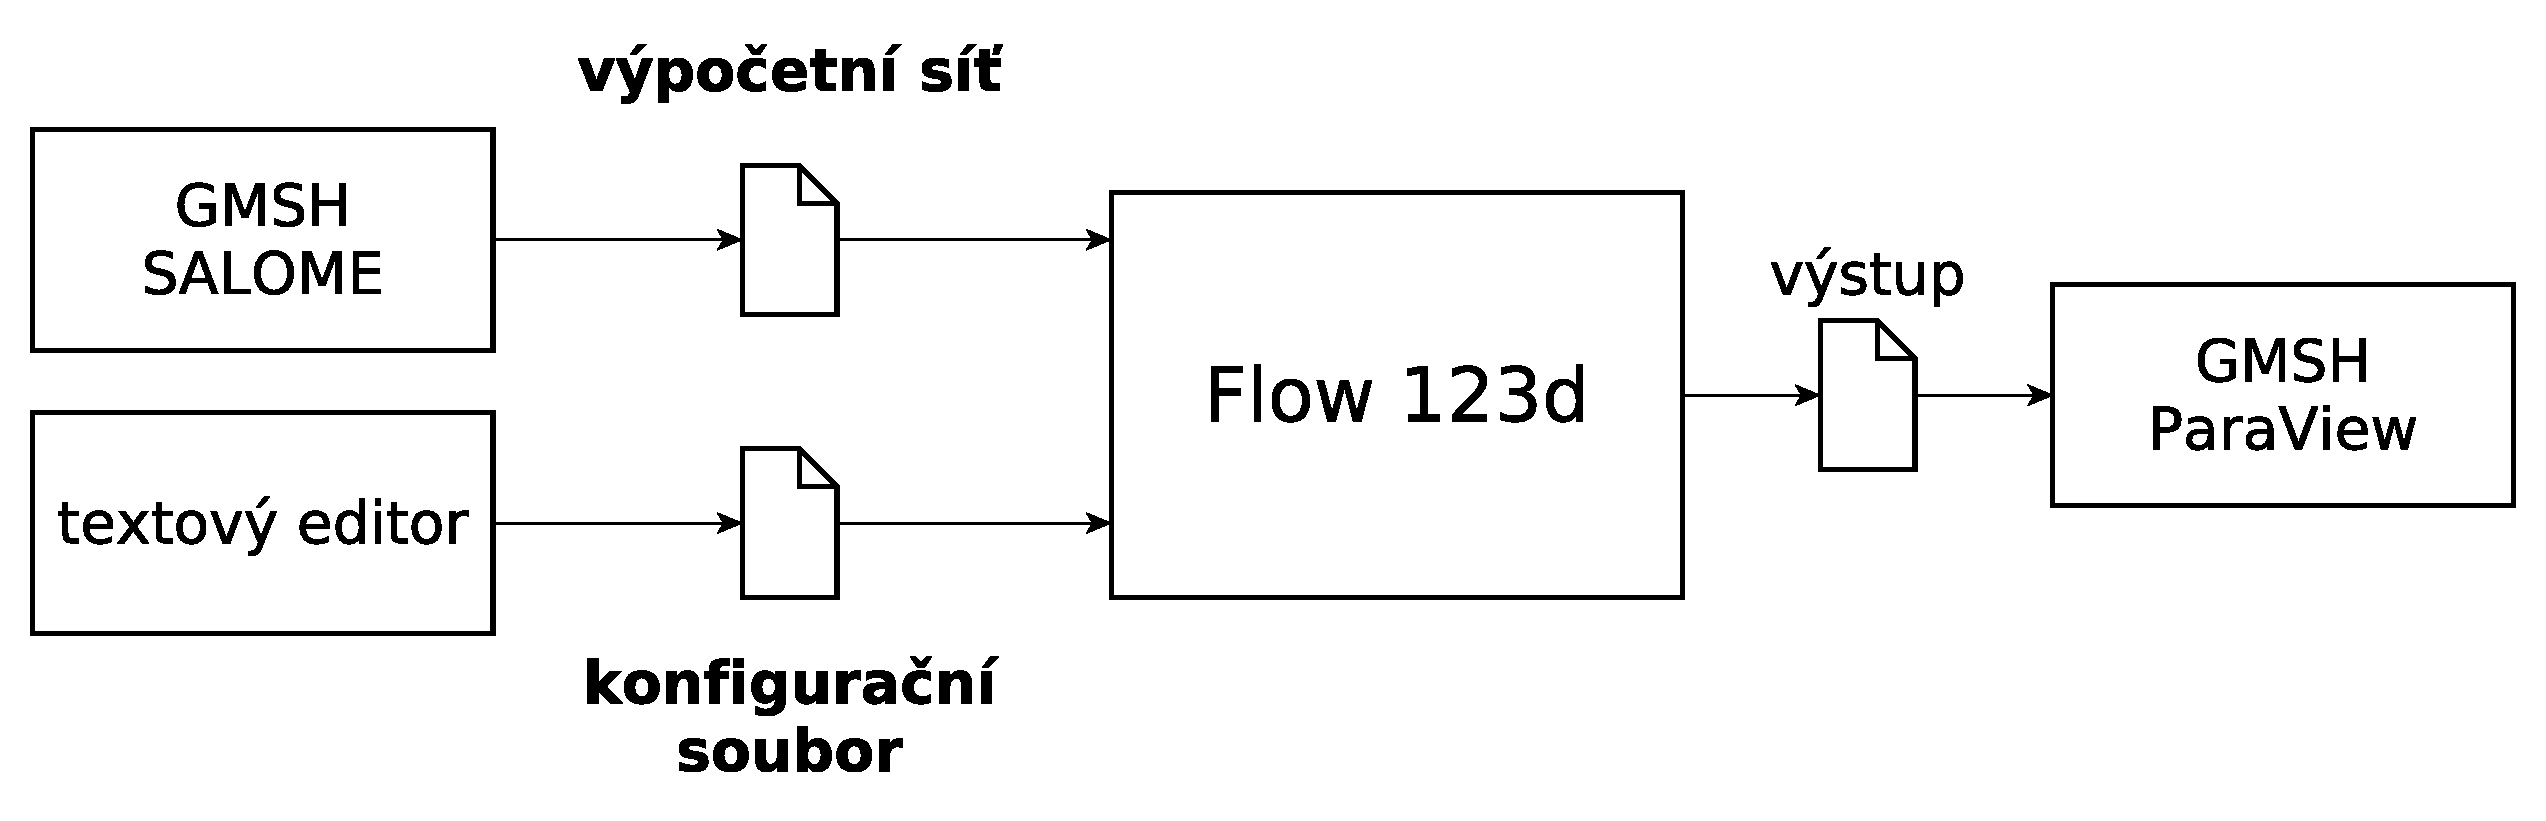
\includegraphics[width=\textwidth]{../../img/flow123d_presentation.png}
}
	\only<4>{\transparent{1}
	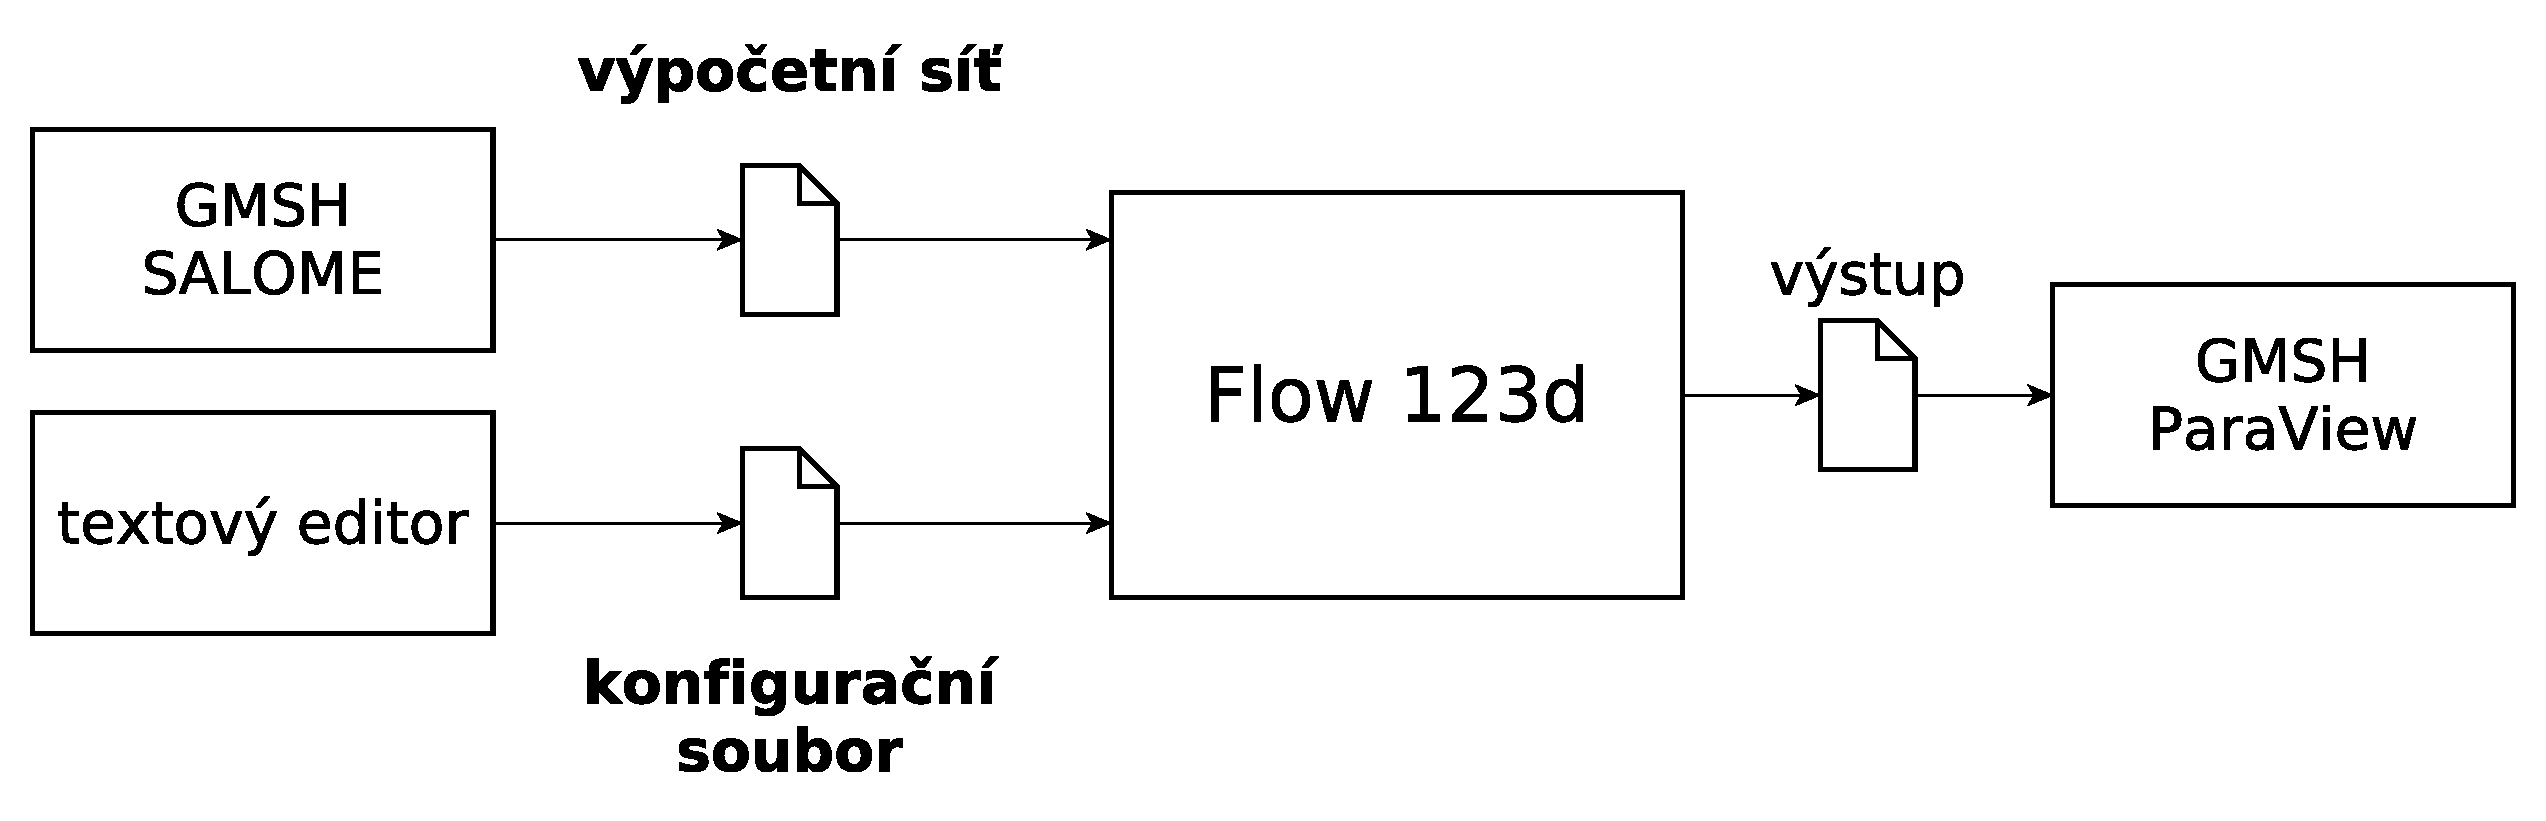
\includegraphics[width=\textwidth]{../../img/flow123d_presentation.png}
	}
	\end{figure}
\end{frame}

\begin{frame}
	\frametitle{Zadávání výpočetních úloh}
	\begin{itemize}[<+>]
		\item textový soubor ve formátu CON (JSON)
		\item inicializace úlohy ve Flow123d
		\item různé typy úloh
		\item rozsáhlá specifikace formátu
		\item konfigurační soubor píšou uživatelé
	\end{itemize}
\end{frame}

\begin{frame}[fragile]
	\frametitle{Problémy s konfiguračními soubory}
	Syntaxe
	\begin{itemize}
		\item<2> uzávorkování vnořených výrazů
		\item<3> oddělovací čárky
		\item<4> uvozovky
	\end{itemize}

\vspace*{-0.5cm}
\begin{figure}[ht]
\begin{minipage}[t]{0.45\linewidth}
\begin{exampleblock}{Formát CON}<1->
\begin{lstlisting}
output = {
  output_stream = {
    file = "out.pvd", 
    format = {
      TYPE = "vtk", 
      variant = "ascii"
    }, 
    name = "out_stream"
  }
}
\end{lstlisting}
\end{exampleblock}
\end{minipage}
\begin{minipage}[t]{0.45\linewidth}
\begin{exampleblock}{Formát YAML}<5>
\begin{lstlisting}
output:
  output_stream:
  	file: out.pvd
  	format: !vtk
  	  variant: ascii
  	name: out_stream
\end{lstlisting}
\end{exampleblock}
\end{minipage}
\end{figure}	
\end{frame}


\begin{frame}
	\frametitle{Problémy s konfiguračními soubory}
	\begin{itemize}
	\item<1-5> Je úloha správně zadána?
	\begin{itemize}
		\item<2,6-> verze Flow123d
		\item<3,6-> správná datová struktura
		\item<4,6-> povinné klíče a atributy pro vybranou úlohu
		\item<5,6-> správný počet prvků v poli
	\end{itemize}
	\item<6-9> chyba v konfiguračním souboru
		\begin{itemize}
			\item<-5,7> textové rozhraní Flow123d
			\item<-5,8> rozsáhlá referenční dokumentace
			\item<-5,9> vzdálené spouštění
		\end{itemize}
	\end{itemize}
\end{frame}

\begin{frame}
	\frametitle{Editor konfiguračních souborů}
	\begin{itemize}
		\item<1> grafický nástroj pro práci konfiguračními soubory
		\item<2> formát YAML
		\item<3> validace konfiguračního souboru
		\item<4> kontextová dokumentace
		\item<5> automatické doplňování textu
		\item<6> základní funkce textového editoru
	\end{itemize}
\end{frame}

\begin{frame}{}{}
\begin{center}
\huge Děkuji za pozornost.
\end{center}
\end{frame}


\end{document}
